\documentclass{beamer}

\usepackage[T1]{fontenc}
\usepackage[utf8]{inputenc}
\usepackage[ngerman]{babel}

% Schriftart
\usepackage{mathptmx}
\usepackage[scaled=.90]{helvet}
\usepackage{courier}
\usepackage{verbatim}   % useful for program listings

\usepackage{tikz}
\usetikzlibrary{arrows, shapes.arrows}

% Design wählen
\usetheme[secheader]{Boadilla}

\useinnertheme{rectangles} % Vierecke
\setbeamercovered{invisible} % verdeckten Text komplett ausblenden.

% weitere Einstellungen
\setbeamertemplate{mini frames}[box] % shows small rectangles as mini frames.
%\setbeamersize{text margin left=2em,text margin right=2em}
\setbeamertemplate{sections/subsections in toc}[square]
\setbeamertemplate{bibliography item}[default]
\setbeamertemplate{itemize items}[triangle]
\setbeamertemplate{enumerate items}[square]
\setbeamertemplate{blocks}[rounded][shadow=false]

% Navigation ausblenden
\beamertemplatenavigationsymbolsempty

% Nummerierung bei frame breaks
\setbeamertemplate{frametitle continuation}{(\insertcontinuationcount)}

% Trennfolie vor jedem neuen Kapitel
\AtBeginSection{
  \begin{frame}
    \begin{center}
      \structure{\huge \textsf{\insertsection}}
    \end{center}
  \end{frame}
}

% Zentrierung innerhalb einer Aufzählung
\def\MLine#1{\par\hspace*{-\leftmargin}\parbox{\textwidth}{\[#1\]}}
\def\CLine#1{\par\hspace*{-\leftmargin}\parbox{\textwidth}{#1}}

\title[Extraktion von Entitäten aus Suchergebnisseiten]{Extraktion von Entitäten aus Suchergebnisseiten}
\subtitle{Arbeitsgruppe Informationssysteme}
%\author{GRUPPENBEZEICHNUNG\_kurz}
\institute[Arbeitsgruppe Informationssysteme]{
  Universität Duisburg-Essen\\
  Fakultät für Ingenieurwissenschaften\\
  Abteilung Informatik und Angewandte Kognitionswissenschaft\\
  Arbeitsgruppe Informationssysteme 
}
\date{XX.\,Mai 2015}


\begin{document}
  \maketitle

  \begin{frame}[c]{Übersicht}
    \hfill
    \parbox[t][.55\textheight][c]{0.95\textwidth}{%
      \centering %%% oder vergleichbares
      \tableofcontents
    }
  \end{frame}
  
  \section{Aufgabenstellung}
  \begin{frame}[c]{Heutiger Stand}
  \begin{itemize}
  \item Suchmaschinen bieten keine Übersicht über die gefundene Webseiten.
  \item Die Ergebnismenge besteht aus unstrukturierten Daten.
  \item Es gibt zwar Services, die in der Lage sind, Entitäten zu extrahieren (wie GSA\footnote{\url{http://www.google.com/support/enterprise/static/gsa/docs/admin/70/admin_console_help/crawl_entity_recognition.htm}}
   oder DBpedia spotlight\footnote{\url{http://dbpedia-spotlight.github.io/demo/}}), aber diese Systeme haben folgende Nachteile:
   \begin{itemize}
      \item Die wurden hauptsächlich für englische Sprache entwickelt.
      \item Die Unterstützung des Benutzers bei der Suche wird nicht geleistet.   
   \end{itemize}
  \end{itemize}
  \end{frame}
  
  \begin{frame}[c]{Aufgabenstellung}
  Es soll ein Framework entwickelt werden, das
  \begin{itemize}
  \item Die Extraktion von Entitäten aus deutschen Texten ermöglicht.
  \item Die extrahierte Entitäten mit den Daten aus DBpedia verlinkt.
  \item Die verlinkten Entitäten mithilfe von einer API anderen Programmen zur Verfügung stellt
  \end{itemize}
  Dieses System soll die Benutzerunterstützung bei der Suche ermöglichen.
  \end{frame}
  \section{Lösungskonzept}
  \begin{frame}[c]{Kommunikationsdiagramm}
  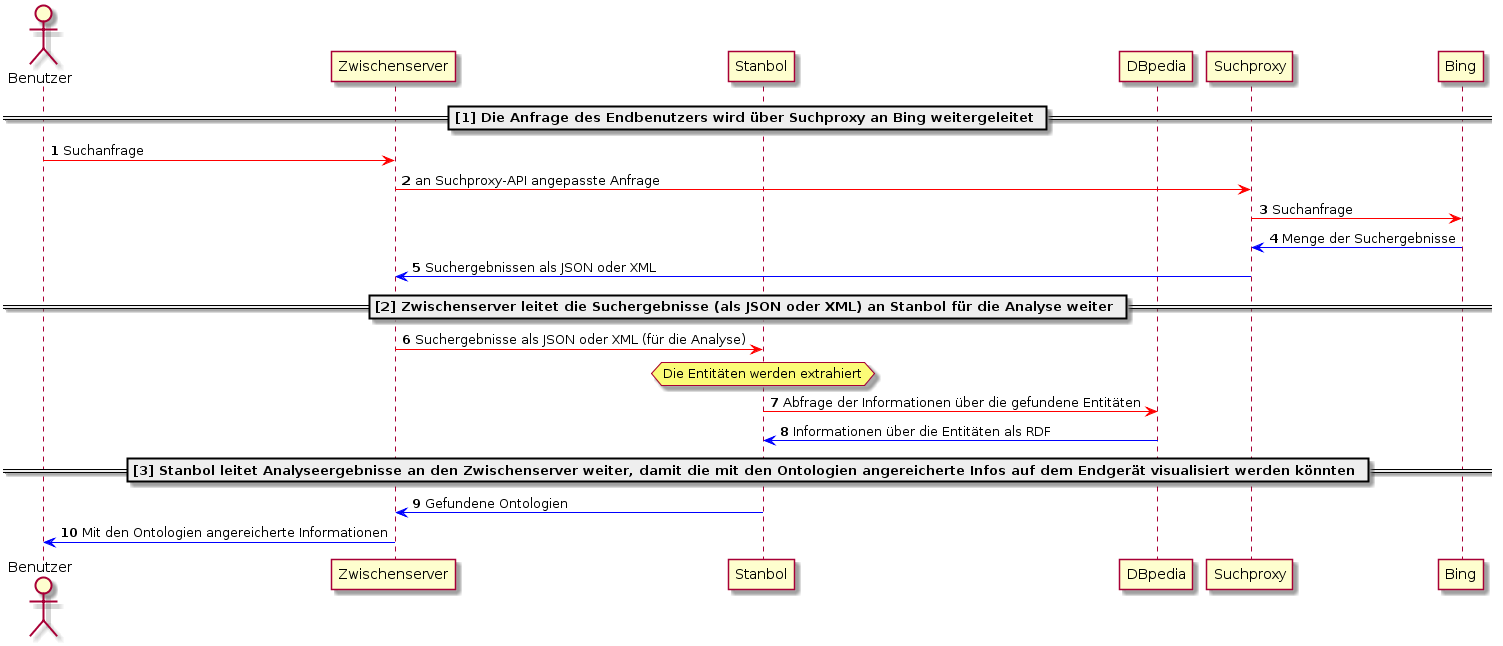
\includegraphics[width=0.94\linewidth]{diagramms/kommunikation.png}
  \end{frame}
  
  \begin{frame}[c]{Funktionsdiagramm des Enchancers}
  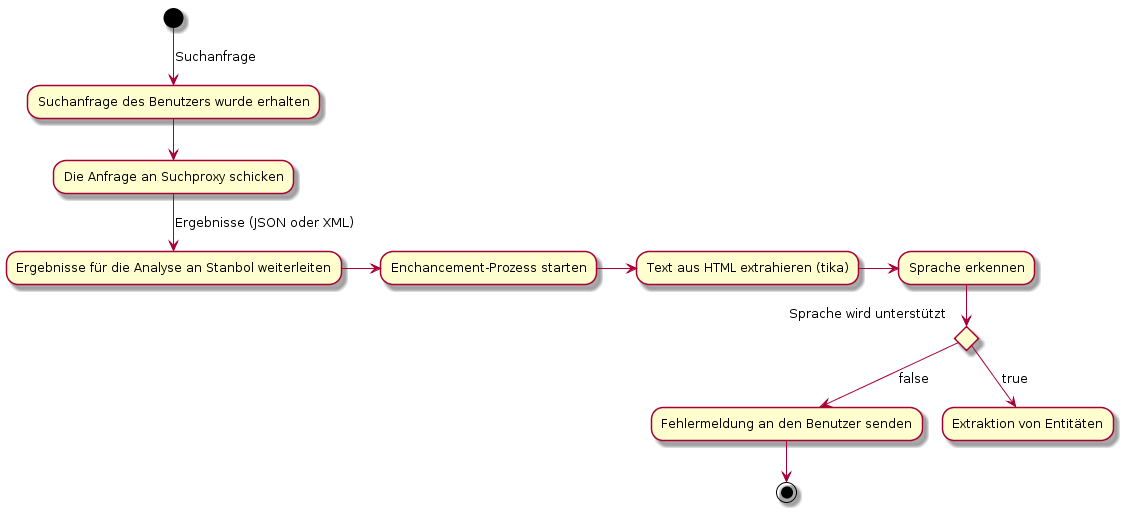
\includegraphics[width=0.45\linewidth]{diagramms/funktionsweise.png}
  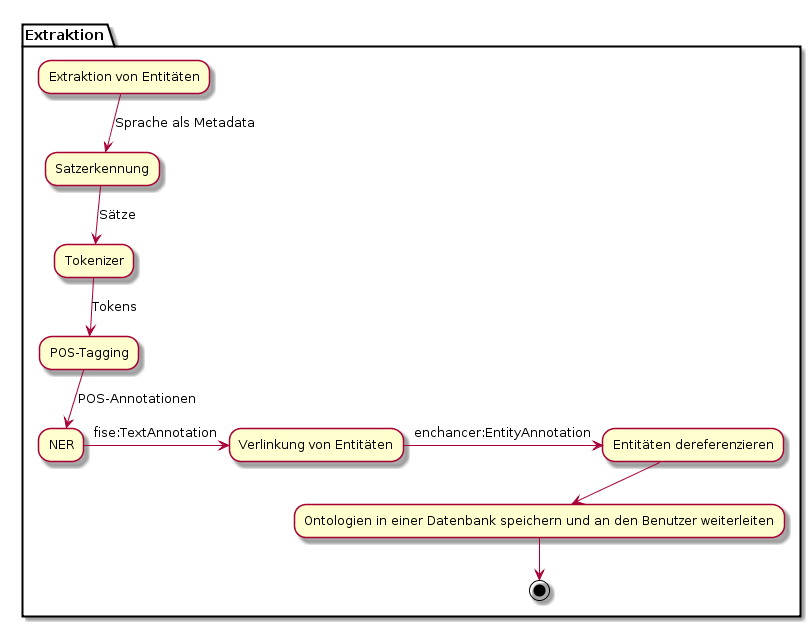
\includegraphics[width=0.55\linewidth]{diagramms/funktionsweise-extraktion.png}
  \end{frame}
  \section{Zeitplan}
  \section{Zusammenfassung}
\end{document}
